
% Lecture Template for ME3023 -  Measurements in Mechanical Systems - Tennessee Technological University
% Spring 2020 - Summer 2020 - Fall 2020 - Spring 2021 - Summer 2021
% Tristan Hill, May 07, 2020 - June 12, 2020 - July 08, 2020 - Novemeber 02, 2020 - March 28, 2021 - May 25, 2021
% Module Name: - Introduction
% Topic 2 - Types of Variables

\documentclass[fleqn]{beamer} % for presentation (has nav buttons at bottom)

\usepackage{/home/thill/Documents/lectures/measurements_lectures/measurements_lectures}

\author{ME3023 - Measurements in Mechanical Systems} % original formatting from Mike Renfro, September 21, 2004

\newcommand{\TNUM}{2\hspace{2mm}} % Topic number 
\newcommand{\moduletitle}{Introduction}
\newcommand{\topictitle}{Types of Variables}

\newcommand{\sectiontitleI}{Measured Variable}
\newcommand{\sectiontitleII}{Independent and Dependent Variables}
\newcommand{\sectiontitleIII}{Controlled Variables and Parameters}
\newcommand{\sectiontitleIV}{Extraneous Variables}
\newcommand{\sectiontitleV}{Engineering Example}

% custom box
\newsavebox{\mybox}

\title{Lecture Module - \moduletitle}

\date{Mechanical Engineering\vspc Tennessee Technological University}


\begin{document}

\lstset{language=MATLAB,basicstyle=\ttfamily\small,showstringspaces=false}

\frame{\titlepage \center\begin{framed}\Large \textbf{Topic \TNUM - \topictitle}\end{framed} \vspace{5mm}}

% Section 0: Outline
\begin{frame}

\large \textbf{Topic \TNUM - \topictitle} \vspace{3mm}\\

\begin{itemize}

	\item \hyperlink{sectionI}{\sectiontitleI} \vspc % Section I
	\item \hyperlink{sectionII}{\sectiontitleII} \vspc % Section II
	\item \hyperlink{sectionIII}{\sectiontitleIII} \vspc %Section III
	\item \hyperlink{sectionIV}{\sectiontitleIV} \vspc %Section IV
	\item \hyperlink{sectionV}\sectiontitleV 	\vspc %Section IV

\end{itemize}

\end{frame}

% Section 1
\section{\sectiontitleI}
\begin{frame}[label=sectionI]
\frametitle{\sectiontitleI}

\large{``A {\BL measurement} is an act of assigning a specific value to a physical variable. That physical variable
is the {\GR measured variable}.''} \vspc
{\tiny Text: Theory and Design of Mech. Meas.}

\end{frame}

% Section 2
\section{\sectiontitleII}
\begin{frame}[label=sectionII]
\frametitle{Independent and Dependent Variables}

{``If a change in one variable will not affect the value of some other variable, the
two are considered independent of each other. A variable that can be changed independently of other
variables is known as an {\PR independent variable}. A variable that is affected by changes in one or more
other variables is known as a {\BR dependent variable}. Normally, the variable that we measure depends on
the value of the variables that control the process.''} \vspc
{\tiny Text: Theory and Design of Mech. Meas.}

\end{frame}

% Section 3
\section{\sectiontitleIII}
\begin{frame}[label=sectionIII]
\frametitle{\sectiontitleIII}

{``A variable is {\BL controlled} if it can be held at a constant value
or at some prescribed condition during a measurement... ...complete control of a variable is not usually
possible. We use the adjective {\BL controlled} to refer to a variable that can be held as prescribed, at
least in a nominal sense... \vspc
...we define a {\GR parameter} as a functional grouping of variables. For example, a moment of inertia or a Reynolds number... ...A {\GR parameter} that has an effect on the behavior of the measured variable is called a control parameter....''} \vspc
{\tiny Text: Theory and Design of Mech. Meas.}

\end{frame}

% Section 4
\section{\sectiontitleIV}
\begin{frame}[label=sectionIV]
\frametitle{\sectiontitleIV}

{``Variables that are not or cannot be controlled during measurement but that affect the value of the
variable measured are called {\RD extraneous variables}. Their influence can confuse the clear relation
between cause and effect in a measurement... ...The effects due to {\RD extraneous variables} can take the form of signals superimposed
onto the measured signal with such forms as {\PR noise} and drift.''} \vspc
{\tiny Text: Theory and Design of Mech. Meas.}

\end{frame}

% Section 5
\section{\sectiontitleV}
\begin{frame}[label=sectionV]
\frametitle{\sectiontitleV}


	\textbf{ SHARP I.R. Ranger - Distance Sensor} \vspc
	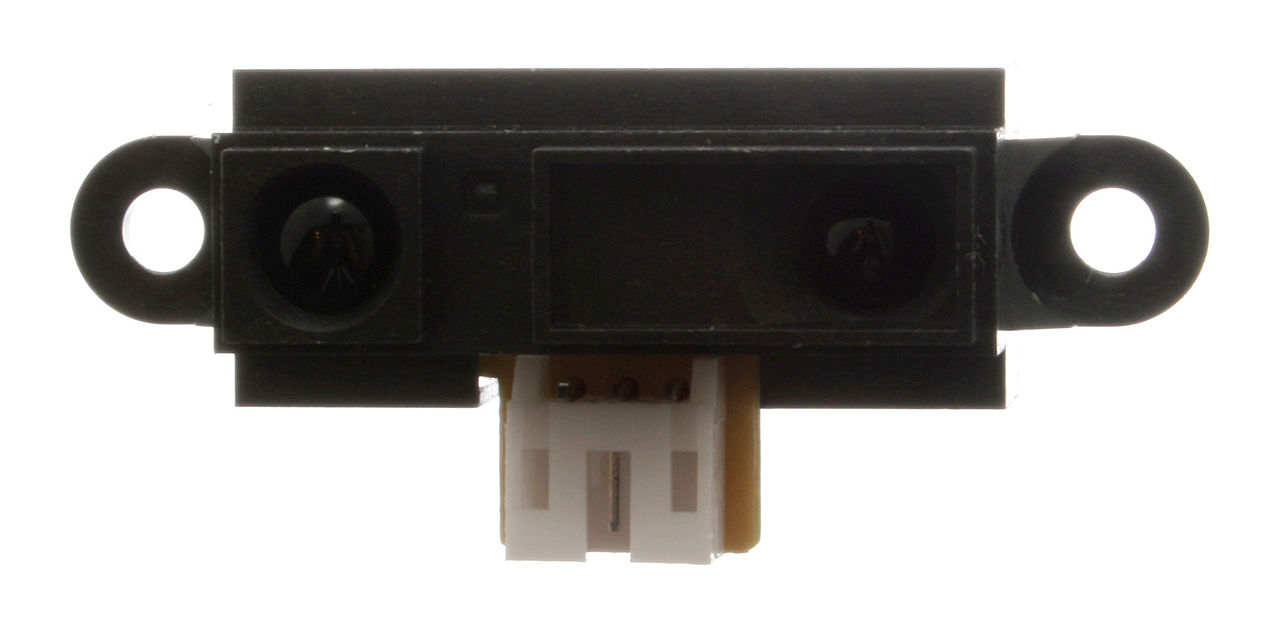
\includegraphics[scale=0.5]{proximity_sensor.jpg} \hspace{20mm}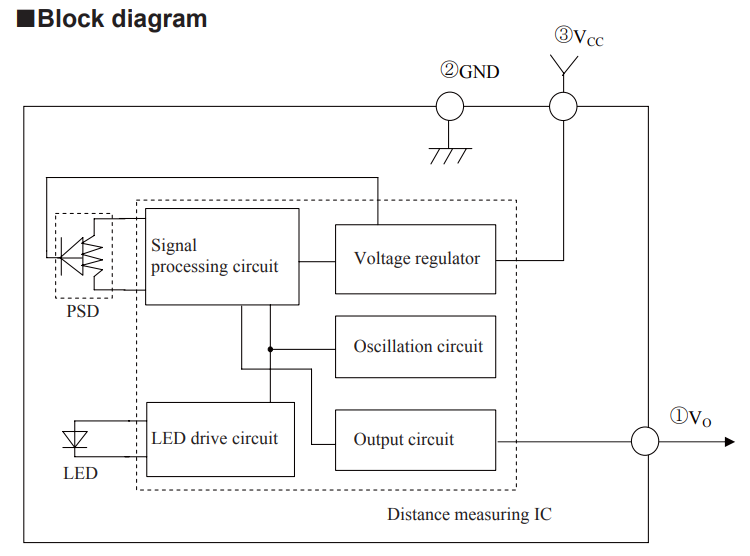
\includegraphics[scale=0.20]{sharp_ranger_circuit.png} \vspc
  {\tiny Image, More Info: \href{https://en.wikipedia.org/wiki/Proximity_sensor}{Wikipedia} }\hspace{40mm} {\tiny Image, More Info: \href{https://en.wikipedia.org/wiki/Position_sensitive_device}{Wikipedia} }

\end{frame}

\begin{frame}
\frametitle{Engineering Example}


Consider the IR distance ranger, name at least one physical variable for each of the following categories. 

\begin{itemize}
	\item Measured Variable \vspc 
	\item Independent Variable \vspc
	\item Dependent Variables  \vspc 
	\item Controlled Variables  \vspc 
	\item Extraneous Variables  \vspc 
\end{itemize}

\end{frame}

\end{document}





